\documentclass[a4paper, 12pt]{article}
\usepackage{geometry}
\geometry{a4paper,
total={170mm,257mm},left=2cm,right=2cm,
top=2cm,bottom=2cm}

\usepackage{mathtext}
\usepackage{amsmath}
\usepackage[T2A]{fontenc}
\usepackage[utf8]{inputenc}
\usepackage[english,russian]{babel}
\usepackage{graphicx, float}
\usepackage{tabularx, colortbl}
\usepackage{caption}
\captionsetup{labelsep=period}

\newcommand{\parag}[1]{\paragraph*{#1:}}
\DeclareSymbolFont{T2Aletters}{T2A}{cmr}{m}{it}
\newcounter{Points}
\setcounter{Points}{1}
\newcommand{\point}{\arabic{Points}. \addtocounter{Points}{1}}
\newcolumntype{C}{>{\centering\arraybackslash}X}

\author{Калинин Даниил, Б01-110}
\date{\today}
\title{Лабораторная работа 4.4.1. Исследование амплитудной решетки}

\begin{document}
\maketitle
\parindent=0cm

\parag {Цель работы}
знакомство с работой и настройкой гониометра Г5, определение спектральных характеристик амплитудной решетки.

\parag {В работе используются}
гониометр, дифракционная решетка, ртутная лампа

\parag {Теоритическая справка} ~\\
Основное соотношение приближенной теории дифракционной решётки:

\begin{equation}
    d\sin \varphi_m = m\lambda.
\end{equation}

Угловая дисперсия $D$ характеризует угловое расстояние между близкими спектральными линиями:

\begin{equation}
    D = \frac{d\varphi}{d\lambda} = \frac{m}{d \cos \varphi}=\frac{m}{\sqrt{d^{2}-m^{2} \lambda^{2}}}.
\end{equation}

\parag {Экспериментальная установка}~\\
При работе с дифракционной решёткой основной задачей является точное измерение углов, при которых наблюдаются главные максимумы для различных длин волн. В нашей работе для измерения углов используется гониометр Г5. Принципиальная схема экспериментальной установки приведена на рис. \ref{img:setup}.

\begin{figure}[h]
    \centering
    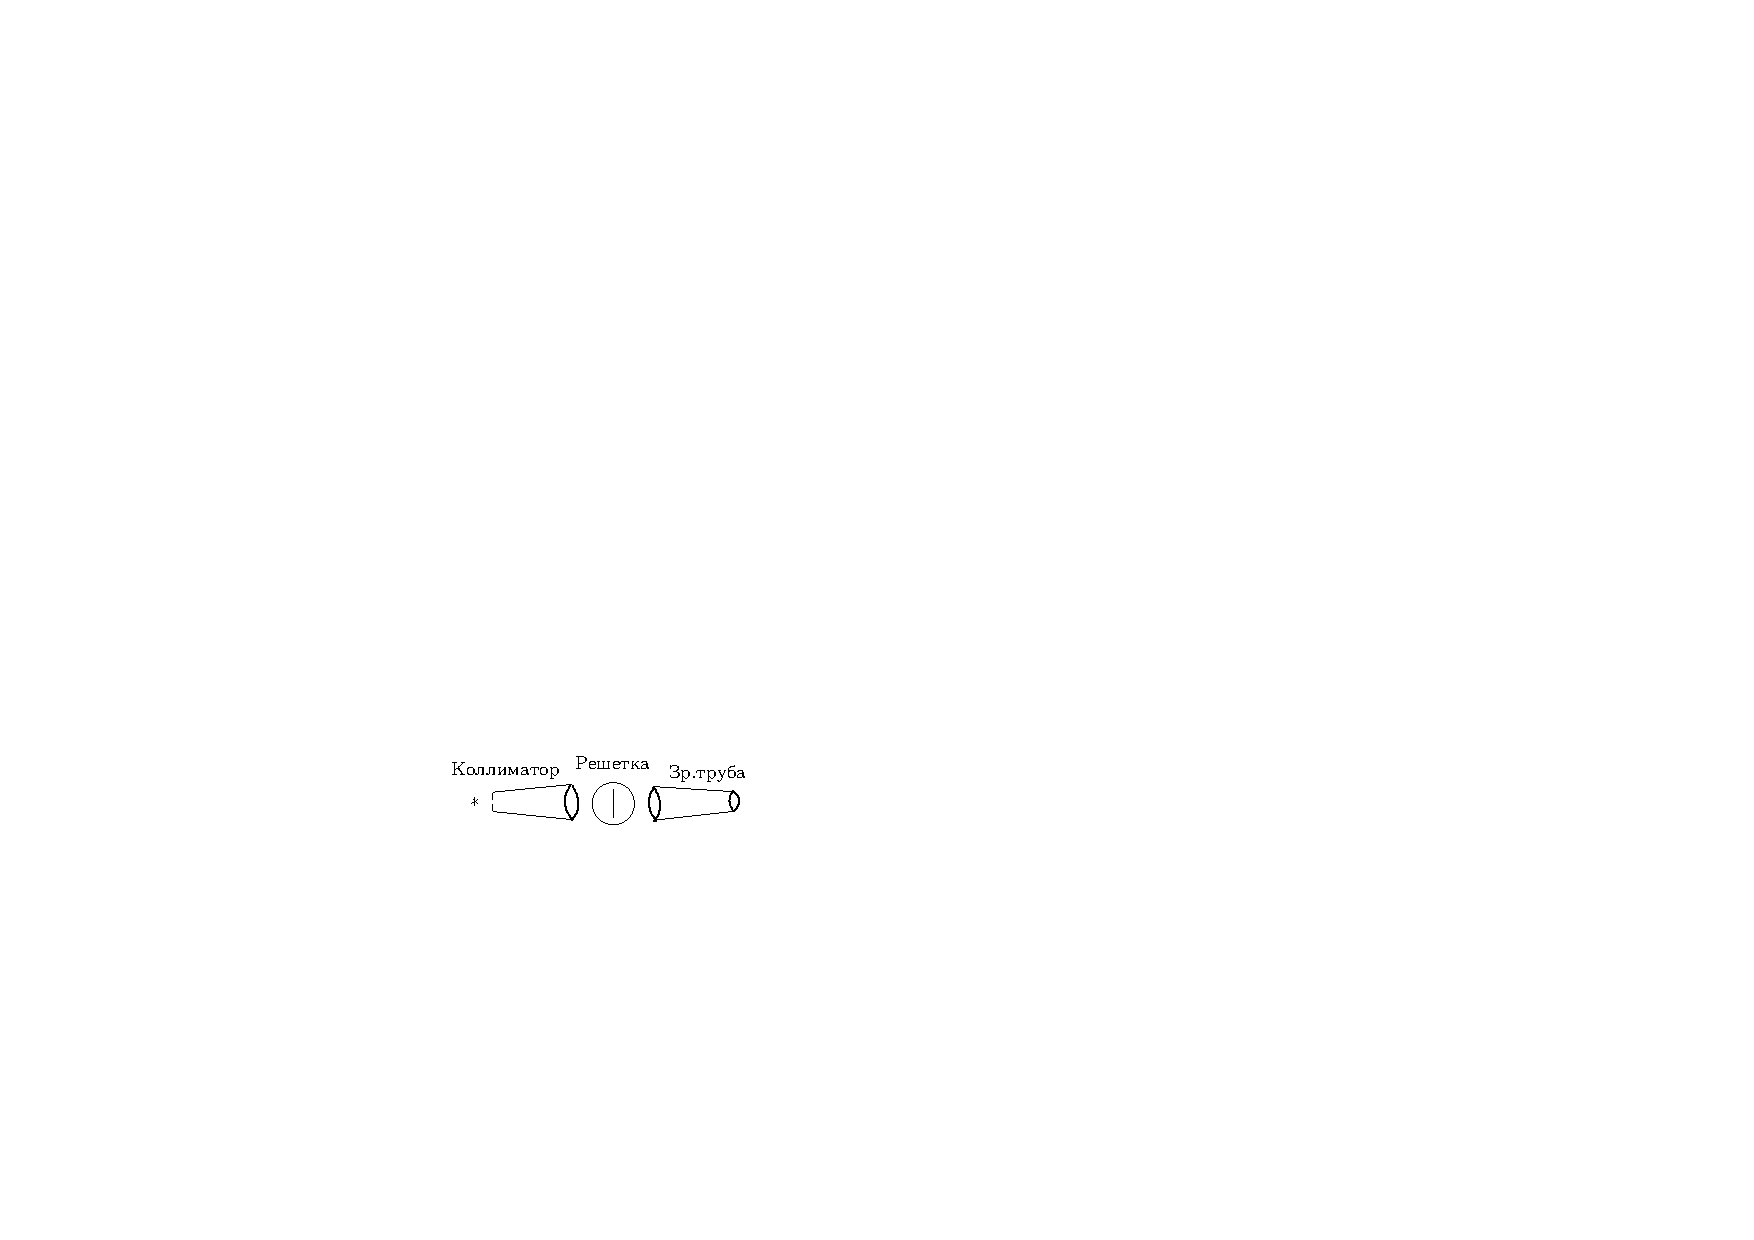
\includegraphics[scale=1.5]{setup.pdf}
    \caption{Схема установки.}
    \label{img:setup}
\end{figure}


\parag {Ход работы} ~\\

\point Измерим координаты спектральных линий ртути в $\pm 1$ порядках. Результаты занесем в таблицу \ref{tabl:expr}.

\begin{table}[h]
\centering
\begin{tabular}{|c|c|c|c|}
\hline 
    Цвет & Длина волны, нм. & угол $\phi_1$, град. & $sin(\phi_1)$ \\ \hline
    фиолетовый & 487.7 & $13^{\circ}36'28''$ & 0.23527 \\ \hline
    синий & 435.8 & $14^{\circ}26'28''$ & 0.24938 \\ \hline
    голубой & 491.6 & $16^{\circ}8'32''$ & 0.27802 \\ \hline
    зеленый & 546.1 & $17^{\circ}45'27''$ & 0.30499 \\ \hline
    желтый & 577.0 & $18^{\circ}40'21''$ & 0.32016 \\ \hline
    желтый & 579.1 & $18^{\circ}44'21''$ & 0.32126 \\ \hline
    
\end{tabular}
\caption{Данные эксперимента}
\label{tabl:expr}
\end{table}
 ~\\

\point Построим график зависимости $\sin(\phi_1)$ от $\lambda$ для $\pm 1$ порядка, изобразим его на рисунке \ref{img:sin_to_lambda}.

\begin{figure}
    \centering
    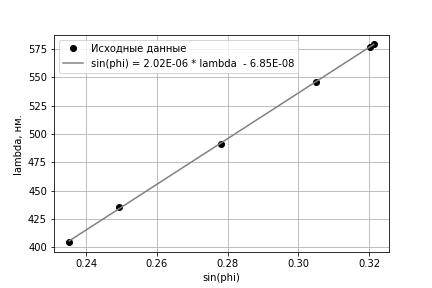
\includegraphics[scale=1]{sin_to_lambda.png}
    \caption{График зависимости $\sin(\phi_1)$ от $\lambda$}
    \label{img:sin_to_lambda}
\end{figure}

По углу наклона графика можно определить период решетки: $d = 2.016 $ мкм.

\point Оценим угловую дисперсию решётки: для этого определим разности угловых координат желтых линий во всех видимых порядках. Результаты занесем в таблицу \ref{tabl:disp}.

\begin{table}[H]
\centering
\begin{tabular}{|c|c|c|c|}
        \hline
        $m$  & $ \Delta \varphi , ''$  & $D$ експеримент.,  $ 10^{-5} $ рад/$  \buildrel _{\circ} \over {\mathrm{A}}$   & $D$ теоретич.,   $ 10^{-5} $ рад/$  \buildrel _{\circ} \over {\mathrm{A}}$   \\ \hline
        1  & 50      & $1,14$   & $5,22$  \\ \hline
        2  & 588     & $13,4$    & $12,2$  \\ \hline
        3  & 1350    & $30,9$    & $29,9$  \\ \hline
       -1  & 239     & $-5,46$   & $-5,22$ \\ \hline 
       -2  & 548     & $-12,5$   & $-12,2$ \\ \hline
       -3  & 1332    & $-30,4$  & $-29,9$ \\ \hline
\end{tabular}
\caption{Угловая дисперсия.}
\label{tabl:disp}
\end{table}

Построим график зависимости $D = f(m)$. Изобразим его на рисунке $\ref{img:d_to_m}$

\begin{figure}
    \centering
    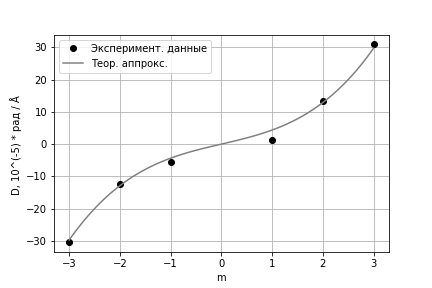
\includegraphics[scale=1]{d_to_m.png}
    \caption{График зависимости $D = f(m)$}
    \label{img:d_to_m}
\end{figure}

\point Получим оценку для разрешимого спектрального интервала $ \delta\lambda $, числа эффективно работающих штрихов решётки $ N $, разрешающей способности $ R $, а также её эффективного размера решетки $ l $:

\begin{equation*}
    \delta\lambda \approx \Delta\varphi/D = 2 \buildrel _{\circ} \over {\mathrm{A}};
\end{equation*}

\begin{equation*}
    R \approx \frac{\lambda}{\delta\lambda} = 2885
\end{equation*}

\begin{equation*}
    N \approx R/m = 2885
\end{equation*}

\begin{equation*}
    l \approx Nd = 6\; \text{мм.}
\end{equation*}

\parag {Заключение} ~\\
В ходе работы были изучены спектральные линии ртути, определен шаг дифракционной решетки, измерена ее угловая дисперсия, а также эффективный размер. Полученные результаты довольно хорошо согласуются с теорией. 
\end{document}
